\newpage
\subsection{Caso d'uso UC14: Amministrazione applicazione web}
\label{UC14}
\begin{figure}[ht]
	\centering
	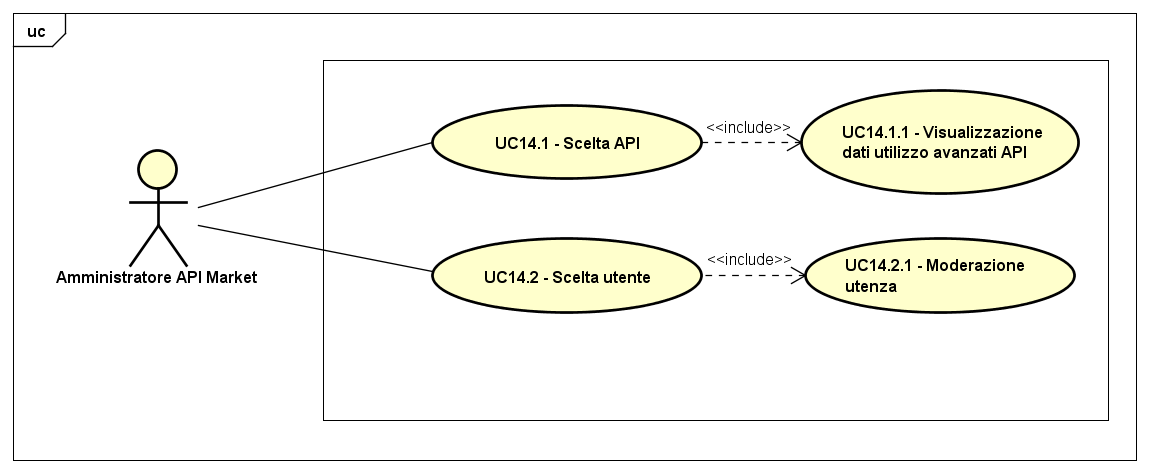
\includegraphics[scale=0.45]{UML/UC14.png}
	\caption{UC13: Amministrazione applicazione web}
\end{figure}

\renewcommand*{\arraystretch}{1.6}
\begin{longtable}{ l | p{11cm}}
	\hline
	\rowcolor{Gray}
	\multicolumn{2}{c}{UC14: Amministrazione applicazione web} \\
	\hline
	\textbf{Attori} & Amministratore API Market \\
	\textbf{Descrizione} & L'attore può gestire la parte riservata della piattaforma, ed effettuare operazioni super-user su utenza, prodotti registrati e sulla piattaforma stessa \\
	\textbf{Pre-Condizioni} & L'attore visita la pagina relativa all'amministrazione della piattaforma API Market\\
	\textbf{Post-Condizioni}& L'attore ha effettuato le modifiche desiderate, o ha consultato i dati desiderati, all'interno della piattaforma\\
	\textbf{Scenario Principale} & \begin{enumerate*}[label=(\arabic*.),itemjoin={\newline}]
		\item L'attore può consultare i dati di utilizzo avanzati per un API
		\item L'attore può moderare l'utenza predisponendo sospensioni o cancellazioni
	\end{enumerate*}\\
\end{longtable}


